\section{Présentation du Laboratoire d' Informatique de Paris 6}
	\subsection{Le laboratoire}
	Le LIP6 est un laboratoire de recherche sous tutelle de l'Université Pierre et Marie Curie, et du CNRS (UMR 7606). Avec 184 chercheurs permanents et 258 doctorants, il est l'un des principaux laboratoires de recherche en informatique en France. Le Directeur du laboratoire est Patrick Gallinari et le directeur adjoint est Pierre Sens. Le laboratoire vient de revenir à Jussieu après plusieurs années d'exil sur le site de Radio France Avenue de Président Kennedy dans le 16° arrondissement.\\
	Le laboratoire couvre un large spectre d'activités regroupées au sein de cinq départements : Calcul Scientifique, Décision, Systèmes Intelligents Recherche opérationnelle, Données et Apprentissage Artificiel, Réseaux et Systèmes Répartis, Systèmes Embarqués sur Puce. En complément de la recherche académique, le LIP6 a une longue tradition de coopération avec des partenaires industriels dans de très nombreux projets nationaux, européens ou internationaux. Deux centres Recherche et Développement  ont été créés : le CERME, Centre Européen de Recherche en Micro-Electronique sur les systèmes embarqués, et Euronetlab, sur l'internet et les réseaux de télécommunication. Le LIP6 est également impliqué dans les pôles de compétitivité de l'Ile-de-France : Cap Digital sur le contenu numérique et System@tic sur les systèmes embarqués.\\
	Il a également des équipes communes avec l'INRIA sur les thématiques du calcul formel et des systèmes répartis, dont l'équipe REGAL qui m'accueille pour ce stage. La coopération internationale est une constante pour les activités du laboratoire. Le LIP6 est membre de plusieurs réseaux d'excellence et développe également des relations suivies avec des universités au Brésil, aux États-Unis, au Japon, et dans de nombreux pays européens. Le laboratoire est largement ouvert aux projets de coopération et à l'accueil de visiteurs scientifiques. Le laboratoire est impliqué dans des enseignements liés à la recherche, qui sont dispensés au Master « Sciences et technologie » à l'Université Pierre et Marie Curie. L'EDITE de Paris (Ecole Doctorale d'Informatique, Télécommunication et Electronique de Paris) accueille nos doctorants.\\


	\subsection{L'équipe REGAL}
	L'équipe REGAL fait partie du département "Réseaux et Systèmes Répartis" qui est dirigé par Bertil Folliot. Le département "Réseaux et Systèmes Répartis" se concentre sur la conception de solutions pour construire et gérer les réseaux et systèmes du futur. Il est constitué de quatre équipes : MoVe (Modélisation et Vérification), REGAL (Répartition et Gestion des Applications à Large Echelle), NPA (Networks and Performances Analysis) et Phare. L'équipe REGAL est un équipe commune avec l'INRIA Rocquencourt, le responsable de cette équipe est Pierre Sens. L'objectif de l'équipe est la gestion de ressources dans le cadre très dynamique de grands réseaux. L'équipe REGAL s'intéresse aux techniques de déploiement d'applications (code et données) adaptées aux environnements extrêmement distribués de grande taille (nombre de processeurs, distances), fortement dynamiques, hétérogènes, sans possibilité simple de gestion centralisée et/ou instantanée de la connaissance mutuelle. L'approche de REGAL repose sur des techniques de réplication et d'adaptation dynamique dans lesquelles un code applicatif et ses données sont dupliqués sur plusieurs sites ce qui permet de tolérer les fautes, d'augmenter la disponibilité et réduire les temps d'accès du service rendu par l'application. Nous étudions la façon dont les systèmes peuvent garantir une qualité de service en termes de fiabilité, disponibilité et cohérence.

	\vspace{1.5cm}
        \begin{figure}[!h]
        \centering
        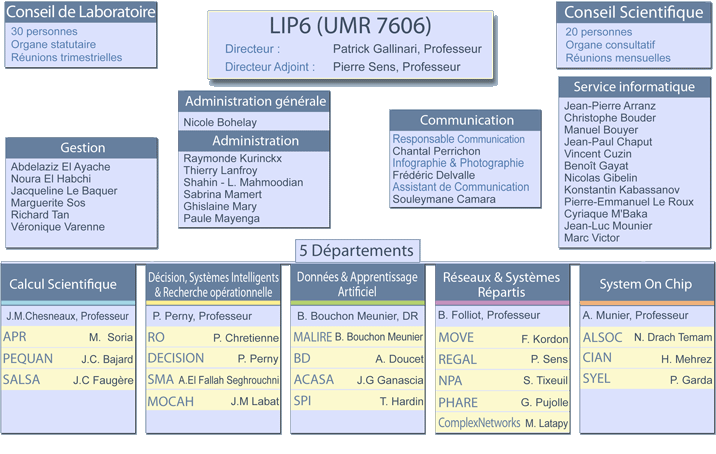
\includegraphics[width=15cm,height=8cm]{../Images/Lip6_Organisation.png}\\
        \caption{Schéma de l'organisation du LIP 6}
        \label{LIP 6}
        \end{figure}
	\vspace{1.5cm}

	\subsection{L'INRIA Paris - Rocquencourt}
	L’INRIA Paris - Rocquencourt est l'un des huit centres de recherche de l’Institut National de Recherche en Informatique et Automatique (INRIA), organisme de recherche spécialisé dans le domaine des Sciences et Technologies de l’Information et de la Communication. C'est un établissement public placé sous la double tutelle du ministère de la recherche et du ministère de l’économie, des finances et de l’industrie, l'INRIA accueille environ 3 800 personnes dont 2 800 scientifiques. \\
	Combiner l’excellence scientifique et le transfert technologique est le fondement de la stratégie de l’institut, dans laquelle s’inscrit en particulier le centre de recherche INRIA Paris - Rocquencourt. Ainsi, ses objectifs prioritaires de recherche - réseaux et systèmes de communication - logiciels fiables et sécurité - modélisation du vivant et de l'environnement – sont conduits avec le souci de concilier recherche en amont du meilleur niveau international, applications et valorisation par le biais d’interactions constantes avec le monde socio-économique.\\
	Ils mènent ses activités scientifiques en développant des partenariats étroits avec les équipes internationales de pointe, le monde de l’industrie et des services, en particulier dans le cadre des pôles de compétitivité, et de nombreux établissements d’enseignement supérieur et de recherche d’Île-de-France.
	
